\documentclass[11pt]{article}
\usepackage[margin=2.5cm]{geometry}
\usepackage[T1]{fontenc}
\usepackage[utf8]{inputenc}
\usepackage{lmodern}
\usepackage{amsmath}
\usepackage{siunitx}
\usepackage{graphicx}
\usepackage{booktabs}
\usepackage[numbers,sort&compress]{natbib}
\usepackage[hidelinks]{hyperref}
\usepackage{caption}
\captionsetup{font=small,labelfont=bf}
\graphicspath{{figures/}{../assets/figures/}}
\sisetup{group-separator={\,},group-minimum-digits=4}

\title{Natural frequencies and transient impact response of a 3D-printed carbon-fibre PETG fan housing,
with an unmeasured elastic modulus}
\author{Cl\'ement Dumeril\thanks{University of California, Berkeley (MEng). Work carried out in June 2026 at
Polytechnia, an engineering consultancy co-founded by the author; convergence study and extended impact runs in
October 2026. Repository: \url{https://github.com/clementdumeril/ventilator-modal-analysis-petgcf}.}}
\date{October 2026}

\begin{document}
\maketitle

\begin{abstract}
The housing of a desk fan printed in carbon-fibre PETG (PETG-CF) is analysed with code\_aster for resonance with
the rotor and for its response to an impact. The free-free modes, with the motor and electronics as distributed masses,
were first computed with linear tetrahedra; a convergence study shows these to be 12 to \SI{20}{\%} too stiff, while
quadratic tetrahedra on four meshes agree within \SI{1}{\%}, at 44.0, 64.3 and \SI{109.9}{Hz} for the first three
modes with $E=\SI{6}{GPa}$. The Young's modulus of the printed material is not measured. Between \SI{3.8}{GPa}, the
published value for printed PETG with \SI{30}{\%} carbon fibre, and the \SI{6.0}{GPa} of the original model, modes 3, 4
and 5 cross the third and fourth rotor harmonics and the blade-passing frequency at \SI{2000}{rpm}, so a resonance
cannot be ruled out. Three impact cases, a \SI{251}{g}, \SI{2.5}{ms} pulse with the
contact patch held fixed, are run to \SI{30}{ms} with linear transient dynamics and Rayleigh damping; verification
found that the original oblique case fixed a slice through the housing, and it was replaced. With quadratic elements
and a nominal \SI{5}{\%} damping (2 to \SI{5}{\%} over the frequencies involved), the peak von Mises stresses away from
the contact, 114 to \SI{174}{MPa}, sit at junctions of the support arms and the stand and exceed the strength reported
for printed PETG-CF; they are local (95th percentile below \SI{23}{MPa}) and sensitive to the element order and to
the simplified geometry of these junctions.
\end{abstract}

\section{Introduction}

Small rotating machines printed in fibre-reinforced polymers, such as desk fans, drone frames and robot covers, need
two quick structural checks before a first print: whether a natural frequency of the printed part sits on an
excitation line of the rotor, and where the part concentrates stress when it is knocked over. Both are routine with
finite elements, but for a printed composite the inputs are uncertain. Fused-filament parts are anisotropic and
weaker between layers \citep{ahn2002}, and short carbon fibres raise the stiffness by an amount that depends on fibre
content and print orientation \citep{tekinalp2014,prabhakaran2025,batista2023}.

This study covers the housing of a desk fan designed at Polytechnia: a cylindrical shroud on a stand, printed in
carbon-fibre PETG (PETG-CF), carrying a brushless motor in the shroud and the electronics in the base. The rotor has five
blades and runs at a nominal speed of \SI{2000}{rpm} in this study. The contributions are:
\begin{itemize}
  \item a free-free modal model of the housing with the motor and electronics as distributed masses, checked against
    the rotor harmonics, with the unmeasured Young's modulus carried as an uncertainty band rather than a single value;
  \item a mesh and element-order convergence study of the first modes, missing from the original analysis;
  \item a linear transient analysis of three impact cases, with damping, run past the end of the load pulse to the
    peak response, with stress metrics that separate the boundary-condition singularity at the contact from the stress
    in the housing, and a check of the contact patches that corrects one of the original cases.
\end{itemize}

\section{Related work}

The anisotropy of fused-deposition parts was characterised early by \citet{ahn2002}: strength and stiffness depend on
raster orientation and drop across layers. Carbon-fibre reinforcement of printed polymers raises the in-plane stiffness
when fibres align with the extrusion direction \citep{tekinalp2014}. For PETG-CF printed by fused filament fabrication,
\citet{prabhakaran2025} report a tensile modulus rising from \SI{2.3}{GPa} for pure PETG to \SI{3.8}{GPa} at
\SI{30}{\%} fibre, with natural frequencies of test beams \SIrange{18}{25}{\%} higher; \citet{batista2023} and
\citet{kohn2021} report that print parameters and build orientation change the mechanical response markedly, and that
reinforcement does not always raise strength. The rotor-dynamic check used here is the Campbell diagram: frequencies of
the structure plotted against rotor speed together with the lines $k\,\Omega$ of the rotor harmonics
\citep{genta2005}; for a stationary housing the structural frequencies do not depend on speed. The mesh is generated
with NETGEN \citep{schoberl1997} in SALOME \citep{salome}; modal and transient analyses use code\_aster
\citep{codeaster}, with Newmark's average-acceleration scheme \citep{newmark1959} for the transient runs.

\section{Model}

\subsection{Geometry and mesh}

The housing geometry comes from the Polytechnia FreeCAD model. The original CAD would not take a conforming tetrahedral
mesh because of small faces and intersecting surfaces; it was defeatured (small faces and short edges removed, the
detailed support arms replaced by simple ribs, one body removed from a fusion), which lowered the volume by
\SI{1.4}{\%}, and oriented with the base on the $xy$ plane and the height along $+z$. The reference mesh
(Figure~\ref{fig:mesh}) has \num{95358} nodes and \num{312777} linear tetrahedra (TETRA4), from NETGEN with a minimum
size of \SI{1}{mm}, a maximum size of \SI{10}{mm} and fineness 2.

\begin{figure}[h]
\centering
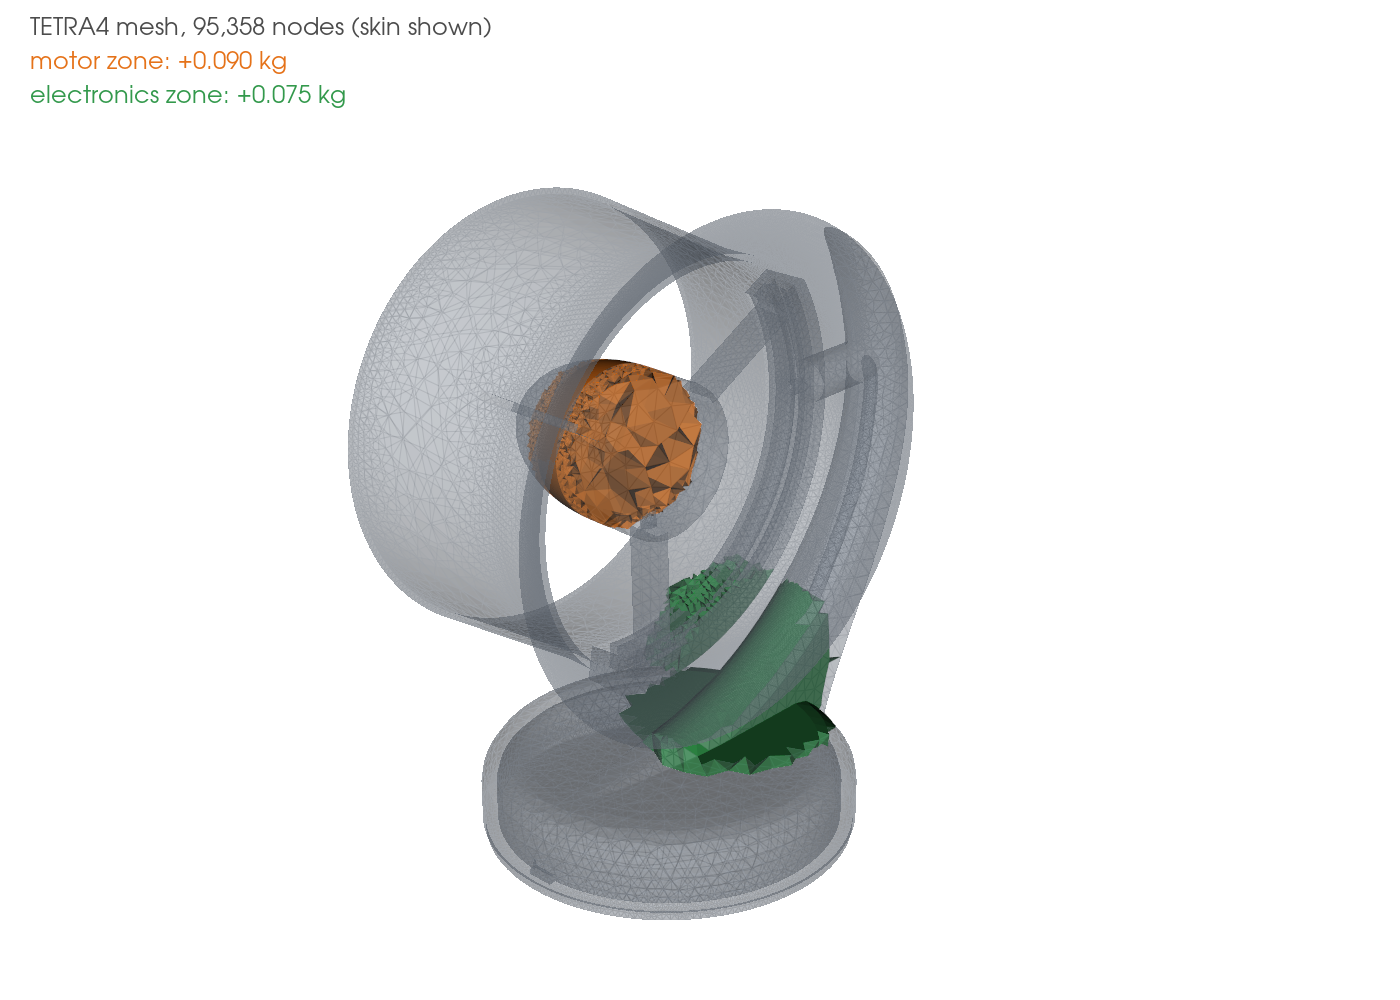
\includegraphics[width=0.48\linewidth]{mesh_mass_zones.png}\hfill
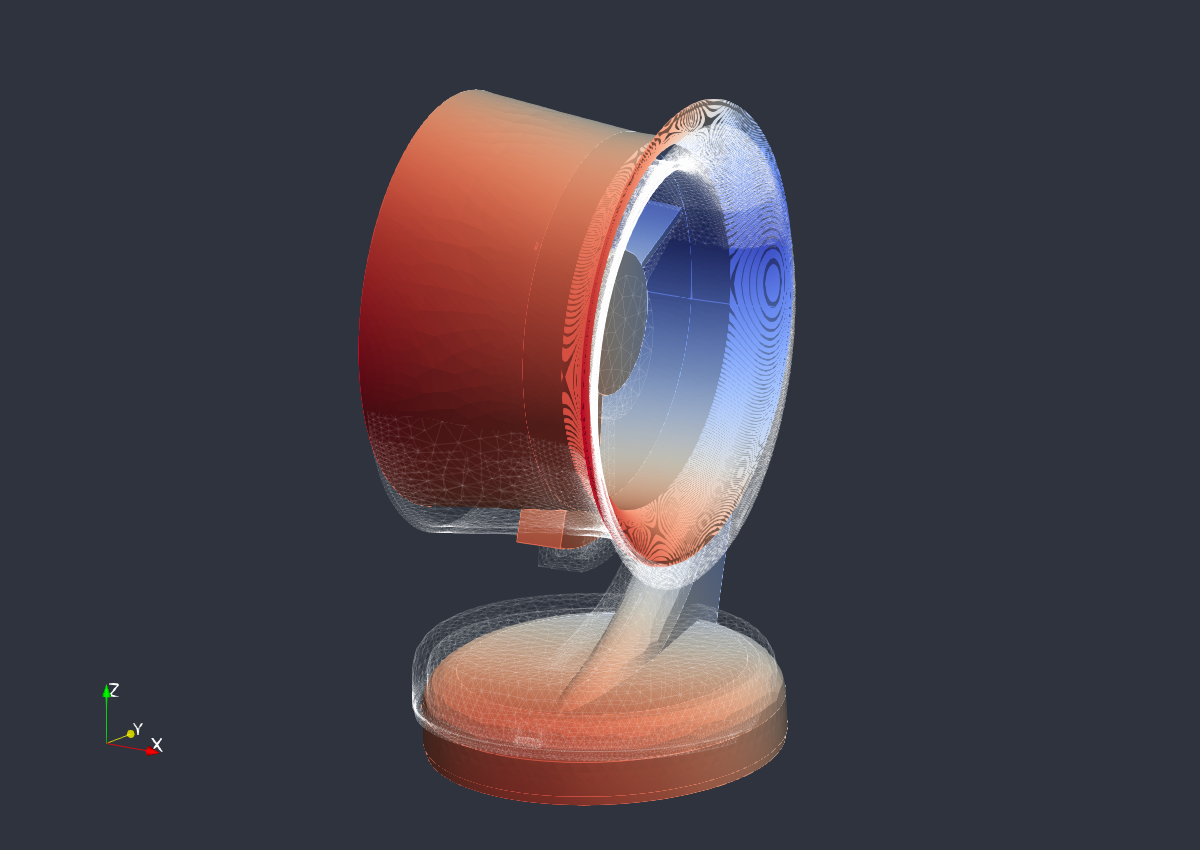
\includegraphics[width=0.48\linewidth]{mode_001_v5_preview.png}
\caption{Left: reference mesh (skin shown) with the motor (orange) and electronics (green) mass zones. Right: first
elastic mode at $E=\SI{6}{GPa}$ (linear-element run of June 2026; deformation amplified).}
\label{fig:mesh}
\end{figure}

\subsection{Material and masses}

PETG-CF is modelled as an isotropic linear-elastic solid (Table~\ref{tab:model}). The density is that of the filament.
The Young's modulus of \SI{6}{GPa} used in the original analysis has no documented source; the published value for
FFF-printed PETG with \SI{30}{\%} carbon fibre is \SI{3.8}{GPa} \citep{prabhakaran2025}. The results below are computed
at \SI{6}{GPa} and carried over the range \SIrange{3.8}{6.0}{GPa}, whose upper bound is only the value of the
original model. The motor (5010 brushless, estimated \SI{0.090}{kg})
and the electronics (controller board, ESC and switch, estimated \SI{0.075}{kg}) are not modelled as solids: their mass
is added to two spherical groups of elements (radius 30 and \SI{45}{mm}, elements with at least half of their nodes
inside) by raising the density there, without adding stiffness. The total mass is \SI{1.080}{kg}.

\begin{table}[h]
\centering
\caption{Model parameters.}
\label{tab:model}
\small
\begin{tabular}{lp{0.68\linewidth}}
\toprule
Quantity & Value \\
\midrule
PETG-CF & isotropic, $E=\SI{6.0}{GPa}$ (range \SIrange{3.8}{6.0}{GPa}), $\nu=0.35$, $\rho=\SI{1300}{kg/m^3}$ \\
Motor zone & sphere $R=\SI{30}{mm}$, \num{23127} elements, $+\SI{0.090}{kg}$ \\
Electronics zone & sphere $R=\SI{45}{mm}$, \num{11616} elements, $+\SI{0.075}{kg}$ \\
Total mass & \SI{1.080446}{kg} \\
Modal boundary conditions & free-free \\
Rotor & 5 blades, nominal \SI{2000}{rpm} ($n=\SI{33.3}{Hz}$, BPF $=\SI{166.7}{Hz}$) \\
Impact pulse & triangular, \SI{2.524}{ms}, peak \SI{2.466e4}{m/s^2} (\SI{251}{g}), $\Delta v=\SI{3.11}{m/s}$ \\
\bottomrule
\end{tabular}
\end{table}

\subsection{Modal problem}

The free-free modes solve $\mathbf{K}\boldsymbol{\phi}=\omega^2\mathbf{M}\boldsymbol{\phi}$. The six rigid-body modes lie
below \SI{1}{Hz}; the search band starts at \SI{1}{Hz}. For an isotropic material at fixed density and Poisson ratio,
$\mathbf{K}$ is proportional to $E$ and the mode shapes do not change, so $f(E)=f(E_0)\sqrt{E/E_0}$ exactly. Each
mode is compared with the rotor lines $k\,n$ ($k=1\dots4$) and with the blade-passing frequency $5n$.

\subsection{Impact model}

The impact is idealised: the nodes of a small patch where the housing touches the floor are held fixed, and the rest
of the housing receives a uniform acceleration pulse $a(t)$ (triangular, \SI{2.524}{ms}, peak \SI{251}{g}). The patch
is the set of nodes within a tolerance of the floor plane, which is tangent to the housing at its extreme point in the
impact direction. In the frame of the patch this is
\begin{equation}
  \mathbf{M}\ddot{\mathbf{u}}+\mathbf{K}\mathbf{u}=-\mathbf{M}\,\mathbf{e}\,a(t),
\end{equation}
with $\mathbf{e}$ the impact direction. The velocity change of the pulse is \SI{3.11}{m/s}, the impact speed of a free
fall of about \SI{0.5}{m} with no rebound. There is no contact law, friction or rebound. Three directions are
studied (Figure~\ref{fig:hotspots}): lateral on the $-y$ side, where the shroud touches the floor (63 fixed nodes,
of the linear mesh, tolerance \SI{3}{mm}); lateral on the $+y$ side, where the stand touches first (63 nodes, \SI{5}{mm}); and oblique, at
\SI{45}{\degree} between $-y$ and $-z$, where the edge of the base touches first (107 nodes, \SI{3}{mm}). The June
study defined the oblique case differently; Section~\ref{sec:verif} explains why it was replaced.

\section{Numerical method}

Modes are computed with \texttt{CALC\_MODES} in a frequency band (shift-invert Lanczos with a Sturm count check),
code\_aster 16.9 for the reference run and 17.4 for the convergence study. The impact runs of June 2026 used
\texttt{DYNA\_NON\_LINE} with an elastic constitutive law up to \SI{2.5}{ms}. Because the problem is linear, the October
runs use \texttt{DYNA\_VIBRA} in the physical basis with the same Newmark average-acceleration scheme
($\beta=1/4$, $\gamma=1/2$), $\Delta t=\SI{0.1}{ms}$, up to \SI{30}{ms}; the system is factorised once, which brings
the cost from about \SI{1000}{s} to \SI{66}{s} of CPU for the first \SI{2.5}{ms}. Stresses are computed at the
archived instants (every \SI{0.2}{ms}). Because the fixed patch creates a stress singularity, the stress is reported as
the maximum, 99th and 95th percentile of the element von Mises stress over the elements whose centroid lies more than
\SI{8}{mm} from the contact plane, next to the raw maximum.

\section{Verification}\label{sec:verif}

\paragraph{Model checks.} The chain was first run with steel properties: scaling the steel first mode
(\SI{125.7}{Hz}) by $\sqrt{E/\rho}$ predicts \SI{52}{Hz} for bare PETG-CF, against \SI{49.2}{Hz} for the June
linear-element model once the \SI{0.165}{kg} of components is added. The mesh volume differs from the prepared CAD by \SI{0.24}{\%}. Recounting the
mass-zone elements from the mesh file gives the same \num{23127} and \num{11616} elements as code\_aster. The Sturm count
finds 21 eigenvalues in \SIrange{1}{1500}{Hz} and 21 modes were computed, with residual norms between
\num{2e-11} and \num{4e-8}. Rotating the model between orientations leaves mode~1 at \SI{49.214}{Hz}.

\paragraph{Mesh and element order.} The June analysis used a single mesh of linear tetrahedra. The convergence study
(Table~\ref{tab:conv}, Figure~\ref{fig:conv}) remeshes the oriented geometry with NETGEN and changes the element order.
Reducing the maximum element size from 10 to \SI{5}{mm} barely changes the mesh (\num{102417} to \num{105816} nodes),
because the element size is set by the thin walls and the curvature, not by the maximum size; refinement was obtained
through the NETGEN fineness instead (\num{123454} and \num{184692} nodes). With linear elements the frequencies keep
falling as the mesh is refined (mode~1 from 49.2 to \SI{46.5}{Hz}, mode~3 from 131.9 to \SI{122.3}{Hz}): linear
tetrahedra are too stiff in the bending of thin walls. Quadratic elements (TETRA10) on four meshes from \num{92381} to
\num{123454} nodes give mode~1 between 43.88 and \SI{44.08}{Hz}, mode~2 between 63.95 and \SI{64.52}{Hz} and mode~3
between 109.44 and \SI{110.27}{Hz}, within \SI{1}{\%}. These meshes are close in size, so they show that the quadratic
results are insensitive to the mesh rather than prove convergence; the spread is not monotonic with refinement and
partly reflects the geometry each mesh captures (total mass 1.0794 to \SI{1.0814}{kg}). An independent estimate comes
from the linear elements: a Richardson extrapolation of the two finest linear meshes, with order 2 in the element size
$h\propto N^{-1/3}$, gives 43.6/64.2/\SI{111.9}{Hz}, within 1 to \SI{2}{\%} of the quadratic values. The first three
frequencies are therefore taken as known to about \SI{2}{\%}, small next to the modulus band. The linear-element values
of the June analysis are 12, 14 and \SI{20}{\%} too high for modes 1, 2 and 3, and the quadratic values on the
reference mesh are used in Section~\ref{sec:res}. The extrapolation does not apply to modes 4 and 5, which are not in
the asymptotic range with linear elements (Section~\ref{sec:res}).

\begin{table}[h]
\centering
\caption{Convergence of the first three elastic modes ($E=\SI{6}{GPa}$). Nodes: corner nodes of the linear mesh. Last row:
Richardson extrapolation of the two finest TETRA4 meshes.}
\label{tab:conv}
\small
\begin{tabular}{lrrrrr}
\toprule
Mesh, element & nodes (corner) & mass (kg) & $f_1$ (Hz) & $f_2$ (Hz) & $f_3$ (Hz) \\
\midrule
published, TETRA4 & 95\,358 & 1.0804 & 49.21 & 73.18 & 131.95 \\
h10, TETRA4 & 102\,417 & 1.0804 & 49.00 & 72.66 & 131.66 \\
fineness 3, TETRA4 & 123\,454 & 1.0814 & 47.37 & 69.80 & 125.49 \\
fineness 4, TETRA4 & 184\,692 & 1.0824 & 46.47 & 68.48 & 122.30 \\
coarse (fineness 1), TETRA10 & 92\,381 & 1.0794 & 43.88 & 63.95 & 109.44 \\
published, TETRA10 & 95\,358 & 1.0804 & 43.97 & 64.29 & 109.87 \\
h10, TETRA10 & 102\,417 & 1.0804 & 43.94 & 64.22 & 109.79 \\
fineness 3, TETRA10 & 123\,454 & 1.0814 & 44.08 & 64.52 & 110.27 \\
\midrule
TETRA4, Richardson ($p=2$) & -- & -- & 43.6 & 64.2 & 111.9 \\
\bottomrule
\end{tabular}

\end{table}

\begin{figure}[h]
\centering
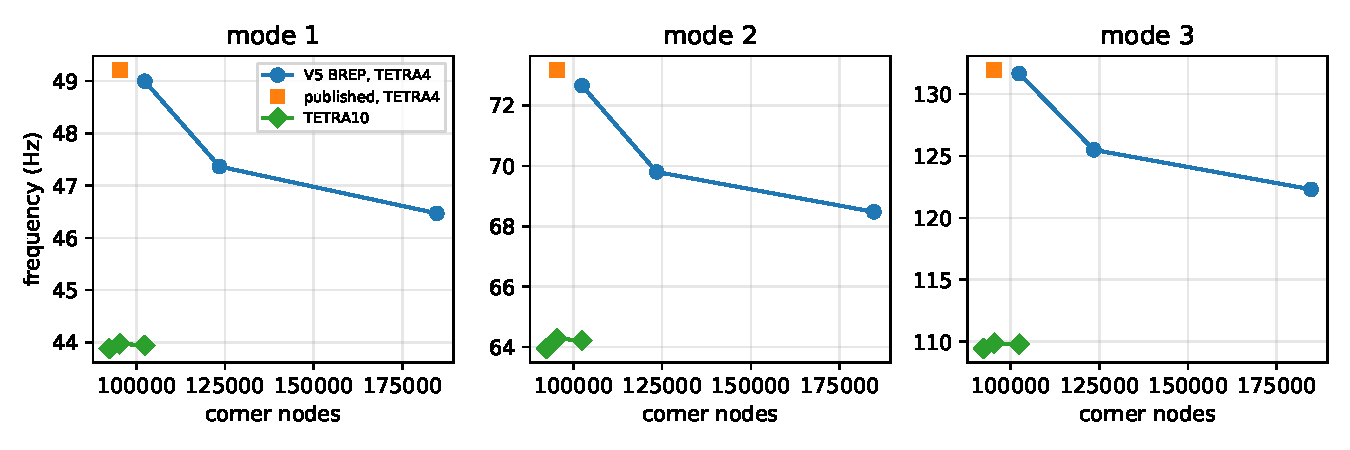
\includegraphics[width=\linewidth]{convergence.pdf}
\caption{Frequencies of modes 1--3 against mesh size: linear tetrahedra (TETRA4) keep falling with refinement;
quadratic tetrahedra (TETRA10) agree within 1\,\% on four meshes; dotted line: Richardson extrapolation of the two
finest TETRA4 meshes.}
\label{fig:conv}
\end{figure}

\paragraph{Transient solver.} The linear solver (\texttt{DYNA\_VIBRA}) reproduces the June non-linear-solver results at
every archived instant up to \SI{2.5}{ms} (identical to four significant digits: \SI{79.82}{MPa}, 95th percentile
\SI{7.070}{MPa}, displacement \SI{4.238}{mm} at \SI{2.5}{ms} for the $-y$ impact). Halving the time step to
\SI{0.05}{ms} on the same case over \SI{15}{ms} changes the stress history by at most \SI{0.4}{\%} and leaves the
peak unchanged (\SI{152.2}{MPa} at \SI{10.8}{ms}; displacement 29.23 against \SI{29.26}{mm}).

\paragraph{Fixed patches.} Plotting the fixed node groups on the mesh showed an error in the June oblique case. Its
plane, with normal $(0,1,1)/\sqrt2$, was placed through the $-y$ side of the shroud and is not tangent to the housing:
the \num{1091} nodes within \SI{1}{mm} of it form a slice through the shroud, the stand and the base, and
\num{17295} nodes lie beyond it. That case fixes a cut through the part rather than a contact patch, and its results
(peak \SI{91}{MPa} in June) are not used. A fall in that direction first touches the edge of the base, at the node that
minimises $y+z$; the corrected oblique case puts the plane through that node. The planes of the two lateral cases are
tangent, with no node beyond them (\path{shock/extended_2026-10/check_contact_planes.py} and its output).

\paragraph{Window length.} Two cases with quadratic elements and $\zeta_n=\SI{5}{\%}$ had not settled at \SI{30}{ms}
and were continued to \SI{60}{ms}: the $-y$ case, whose peak comes at \SI{27.4}{ms}, and the oblique case, whose
response beats. Between 26 and \SI{30}{ms} both reproduce the \SI{30}{ms} runs exactly. After \SI{30}{ms} the
$-y$ case reaches 163~MPa at \SI{36.8}{ms} and at most \SI{121}{MPa} from 40 to \SI{60}{ms}, with the displacement
decaying to \SI{10.7}{mm}; the oblique case reaches at most \SI{118}{MPa}, at \SI{43.8}{ms}. The \SI{30}{ms}
window therefore contains the damped peaks.

\section{Results}\label{sec:res}

\subsection{Modes against the rotor lines}

With quadratic elements, which the convergence study supports (Section~\ref{sec:verif}), the first five elastic modes at
$E=\SI{6}{GPa}$ are 44.0, 64.3, 109.9, 151.8 and \SI{192.1}{Hz} (Figure~\ref{fig:campbell}); the published values,
computed with linear elements, were 12 to \SI{20}{\%} higher for modes 1--3. In mode~1 the shroud moves on its stand
while the base stays nearly still (Figure~\ref{fig:mesh}). At \SI{6}{GPa} no mode sits on a rotor line at
\SI{2000}{rpm}, but mode~2 is \SI{3.6}{\%} below the second harmonic.

Over \SIrange{3.8}{6.0}{GPa} the modes scale by $\sqrt{E/E_0}$:
\begin{itemize}
  \item mode~1 spans \SIrange{35.0}{44.0}{Hz}: above the rotation frequency, but only by \SI{5}{\%} at \SI{3.8}{GPa};
    it would reach the first harmonic at $E=\SI{3.45}{GPa}$, \SI{9}{\%} below the lower bound;
  \item mode~2 spans \SIrange{51.2}{64.3}{Hz}, below the second harmonic over the whole range;
  \item mode~3 spans \SIrange{87.4}{109.9}{Hz} and crosses the third harmonic (\SI{100}{Hz}) at $E=\SI{4.97}{GPa}$;
  \item mode~4 spans \SIrange{120.8}{151.8}{Hz} and crosses the fourth harmonic at $E=\SI{4.63}{GPa}$;
  \item mode~5 spans \SIrange{152.8}{192.1}{Hz} and crosses the blade-passing frequency at $E=\SI{4.52}{GPa}$.
\end{itemize}
Between 4.5 and \SI{5.0}{GPa}, within this range, three modes cross a rotor line. The crossings of modes 4 and 5
exist only with quadratic elements: with linear elements no mode lies between 132 and \SI{228}{Hz}, even on the finest
mesh. Their modes 4 and 5 are at 251 and \SI{290}{Hz} on the reference mesh and still fall quickly with refinement
(228 and \SI{247}{Hz} on the finest mesh); they are probably the quadratic modes 4 and 5, overestimated by 50 to
\SI{65}{\%}, but the mode shapes were not compared. Whether the printed housing
has a resonance at \SI{2000}{rpm} therefore depends on a property that was not measured. Mounting adds a further shift:
the free-free modes ignore the stiffness of whatever the base stands on. A mass-only estimate of the blades,
$f\sqrt{M_0/(M_0+\Delta M)}$ with $M_0=\SI{1.080}{kg}$, lowers every mode by 1 to \SI{6}{\%} for a total blade mass of
25 to \SI{150}{g}; it ignores where that mass sits.

\begin{figure}[h]
\centering
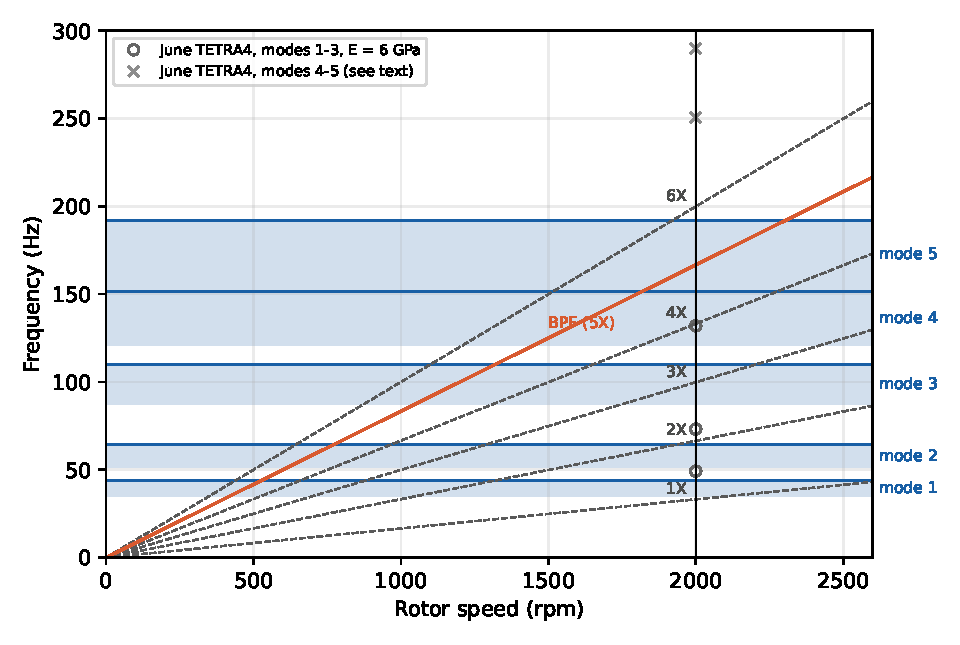
\includegraphics[width=0.75\linewidth]{campbell.pdf}
\caption{Campbell diagram with the TETRA10 modes of the reference mesh. Each band spans the frequency of a mode for
$E=\SI{3.8}{GPa}$ (bottom) to \SI{6.0}{GPa} (top, line). Open circles: June TETRA4 modes 1--3 at \SI{6}{GPa}; crosses:
June TETRA4 modes 4--5, probably the same modes as TETRA10 modes 4--5 (see text). Dashed lines: rotor harmonics; red
line: blade-passing frequency.}
\label{fig:campbell}
\end{figure}

\subsection{Impact}

The June runs stopped at \SI{2.5}{ms}, at the end of the pulse, while the stress was still rising in the two lateral
cases. The October runs continue to \SI{30}{ms} with linear elements at four damping levels and with quadratic elements
undamped and at the central level (Table~\ref{tab:shockall}; the corrected oblique case with quadratic elements at the
central level only). The damping of the printed part is not known, and Rayleigh damping
$\mathbf{C}=\alpha\mathbf{M}+\beta\mathbf{K}$ is assumed, with $\alpha$ and $\beta$ set to give a nominal ratio
$\zeta_n$ of 2, 5 or \SI{10}{\%} at 15 and \SI{300}{Hz}. Between these frequencies the ratio
$\zeta(f)=\alpha/(4\pi f)+\pi\beta f$ is lower, down to $0.43\,\zeta_n$ at \SI{67}{Hz} (Table~\ref{tab:zeta}). For
$\zeta_n=\SI{5}{\%}$ it is \SI{4.6}{\%} at the first mode of the $-y$ case with the patch fixed (\SI{16.6}{Hz}),
\SI{2.4}{\%} at that of the $+y$ case (\SI{42.6}{Hz}), and 2.1 to \SI{2.9}{\%} between 29 and \SI{152}{Hz}. The labels
\SI{2}{\%}, \SI{5}{\%} and \SI{10}{\%} below refer to $\zeta_n$.

\begin{table}[h]
\centering
\caption{Damping ratio of the Rayleigh model, $\zeta(f)$, for the three nominal levels $\zeta_n$ (reached at 15 and
\SI{300}{Hz}). Patch-fixed modes: linear elements.}
\label{tab:zeta}
\small
\begin{tabular}{rlrrr}
\toprule
$f$ (Hz) & & \multicolumn{3}{c}{$\zeta$ (\%) for $\zeta_n=$ 2, 5, 10\,\%} \\
\midrule
15.0 & lower tuning frequency & 2.0 & 5.0 & 10.0 \\
16.6 & mode 1 with the $-y$ patch fixed & 1.8 & 4.6 & 9.1 \\
42.6 & mode 1 with the $+y$ patch fixed & 0.9 & 2.4 & 4.7 \\
44.0 & free-free mode 1 & 0.9 & 2.3 & 4.6 \\
67.1 & minimum of the ratio & 0.9 & 2.1 & 4.3 \\
192.1 & free-free mode 5 & 1.4 & 3.4 & 6.8 \\
300.0 & upper tuning frequency & 2.0 & 5.0 & 10.0 \\
\bottomrule
\end{tabular}

\end{table}

\begin{table}[h]
\centering
\caption{Impact peaks over \SIrange{0}{30}{ms}: von Mises stress $\sigma$ (MPa) more than \SI{8}{mm} from the contact
plane, time of the peak $t$ (ms) and height $z$ (mm) of the peak element, for linear (TETRA4) and quadratic (TETRA10)
elements and nominal Rayleigh ratio $\zeta_n$ (Table~\ref{tab:zeta}). Undamped peaks depend on the length of the
window (see text).}
\label{tab:shockall}
\small
\setlength{\tabcolsep}{4pt}
\begin{tabular}{llrrrrrrrrr}
\toprule
& & \multicolumn{3}{c}{Lateral, Y$-$} & \multicolumn{3}{c}{Lateral, Y+} & \multicolumn{3}{c}{Oblique, base edge} \\
Element & $\zeta$ & $\sigma$ & $t$ & $z$ & $\sigma$ & $t$ & $z$ & $\sigma$ & $t$ & $z$ \\
\midrule
TETRA4 & 0\,\% & 152 & 10.8 & 158 & 123 & 28.4 & 182 & 121 & 11.8 & 158 \\
TETRA4 & 2\,\% & 146 & 10.8 & 158 & 114 & 2.6 & 182 & 117 & 6.2 & 158 \\
TETRA4 & 5\,\% & 138 & 10.8 & 158 & 110 & 2.6 & 182 & 112 & 6.2 & 158 \\
TETRA4 & 10\,\% & 128 & 10.8 & 158 & 104 & 2.6 & 182 & 105 & 6.2 & 158 \\
TETRA10 & 0\,\% & 220 & 27.4 & 198 & 147 & 11.0 & 204 & -- & -- & -- \\
TETRA10 & 5\,\% & 174 & 27.4 & 198 & 114 & 3.0 & 180 & 139 & 8.2 & 158 \\
\bottomrule
\end{tabular}

\end{table}

\paragraph{Undamped response.} Without damping the housing keeps vibrating after the pulse, and the maximum over the
window is set by when the modes happen to add up. With quadratic elements the $-y$ impact shows successive maxima of
171, 172, 179 and \SI{220}{MPa} at 6.6, 13.6, 18.0 and \SI{27.4}{ms}, and the displacement is still rising at \SI{30}{ms}
(\SI{39.8}{mm}): the undamped peak grows with the window and is not used as a result.

\paragraph{Damped response.} With damping the late maxima of the lateral cases disappear, and the peaks sit at junctions
of the housing (Figure~\ref{fig:hotspots}). For the $+y$ impact, where the stand touches the floor, the peak comes at
the end of the pulse (2.6 to \SI{3.0}{ms}) where the upper support arm meets the motor hub. For the $-y$ impact the
housing rocks about the fixed patch (first frequency \SI{16.6}{Hz} with the patch fixed, linear elements) and the peak
comes after the pulse: at \SI{10.8}{ms} with linear elements, where the stand joins the shroud on the side opposite the
impact, and at \SI{27.4}{ms} with quadratic elements, where the upper arm on the impact side meets the shroud. This
late peak comes with the largest rocking displacement (\SI{34.7}{mm} at \SI{29.8}{ms}): it is driven by the rotation of
the whole housing about a patch that stays clamped, which a fan free to bounce or slide would not undergo in this
form, and is probably an artefact of the boundary condition. For the
oblique impact on the base edge the peak is again where the stand joins the shroud, at \SI{6.2}{ms} with linear and
\SI{8.2}{ms} with quadratic elements. With quadratic elements this response beats, with a second maximum of
\SI{136}{MPa} at \SI{25.6}{ms}; continued to \SI{60}{ms}, its later maxima stay lower (at most \SI{118}{MPa}, at
\SI{43.8}{ms}). Damping lowers the peaks slowly: from 152 to \SI{128}{MPa}
between 0 and \SI{10}{\%} for the $-y$ impact with linear elements. Quadratic elements, which are less stiff in bending,
give higher peaks at \SI{5}{\%}: 174 against \SI{138}{MPa} for $-y$, 114 against \SI{110}{MPa} for $+y$ and 139
against \SI{112}{MPa} for the oblique impact. They also move the $-y$ peak to another junction, so the hot spots are
best read as a set of regions (arm-to-hub, arm-to-shroud and stand-to-shroud junctions) rather than as single points.
These peaks are mesh- and geometry-sensitive: the step from linear to quadratic elements raises them by 3 to
\SI{26}{\%} (110 to 114, 112 to 139 and 138 to \SI{174}{MPa}), and they sit at junctions where the detailed arms of
the original CAD were replaced by plain ribs; where such a junction has a sharp re-entrant edge, the computed stress
grows without bound as the mesh is refined. They are therefore not converged values.
The 95th percentile of the stress outside the contact band stays below \SI{26}{MPa} in all runs (\SI{23}{MPa} with
damping), so the peaks are local. The raw maxima, which include the elements at the fixed nodes, reach
\SI{310}{MPa}; inside the contact band they are singularities of the boundary condition.

\begin{figure}[h]
\centering
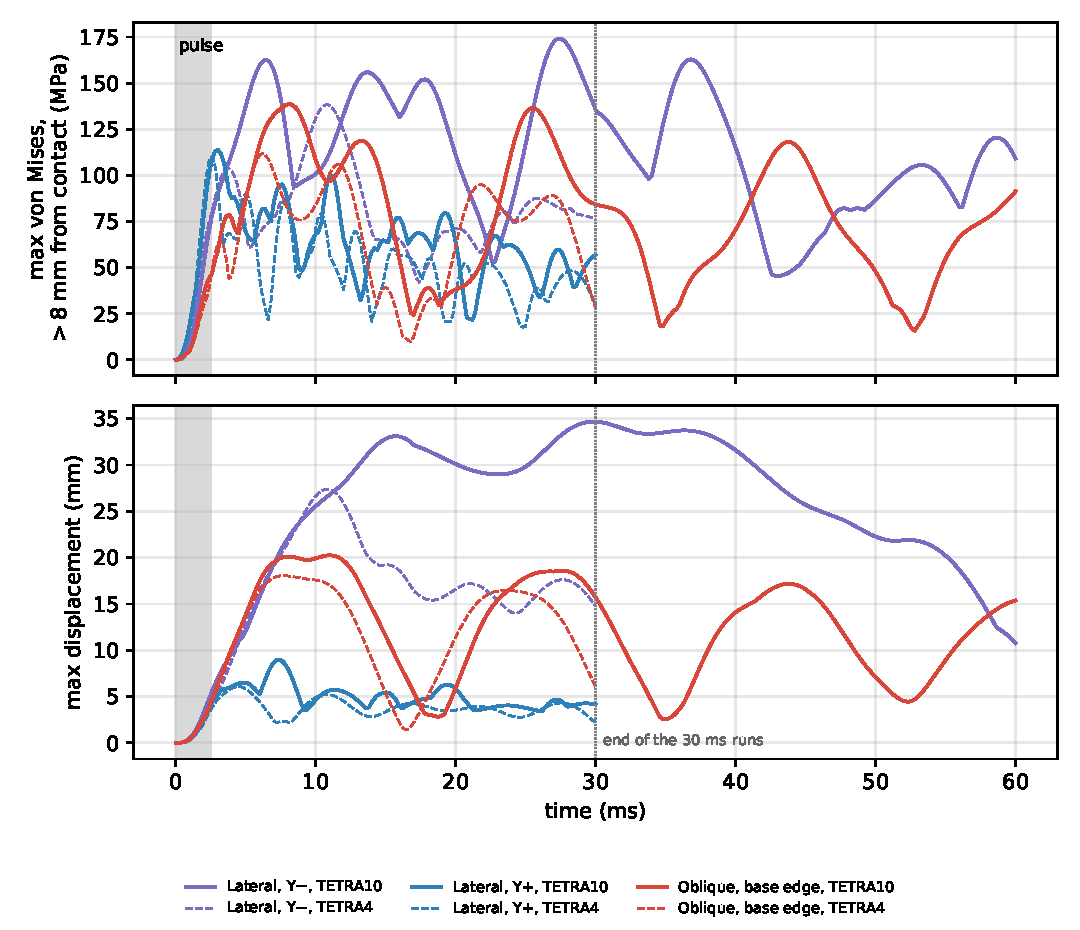
\includegraphics[width=0.82\linewidth]{shock_history.pdf}
\caption{Impact histories at a nominal Rayleigh ratio $\zeta_n=\SI{5}{\%}$: maximum von Mises stress more than \SI{8}{mm} from the
contact plane (top) and maximum displacement (bottom), with quadratic (solid) and linear (dashed) elements. Grey band:
the \SI{2.5}{ms} pulse. Two cases with quadratic elements are continued to \SI{60}{ms}.}
\label{fig:shock}
\end{figure}

\begin{figure}[h]
\centering
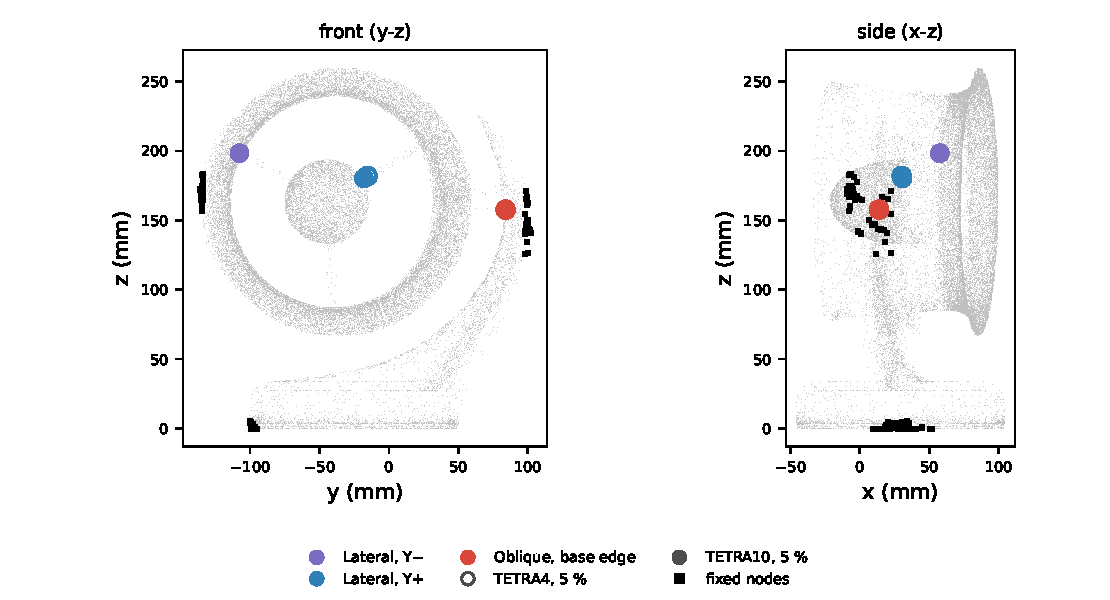
\includegraphics[width=0.9\linewidth]{hotspots.pdf}
\caption{Fixed nodes of the three impact cases (coloured squares) and locations of the peak elements at
$\zeta_n=\SI{5}{\%}$, labelled with the runs that peak there (T4: linear, T10: quadratic elements). A: junction of the
stand with the shroud; B: junction of the upper arm with the hub; C: junction of the upper arm with the shroud, on the
impact side of the $-y$ case. The outline is a random sample of the mesh nodes.}
\label{fig:hotspots}
\end{figure}

\paragraph{Comparison with the material strength.} The tensile strength of FFF-printed PETG with \SI{30}{\%} carbon fibre
is about \SI{60}{MPa} in the plane of the layers \citep{prabhakaran2025}. For unfilled PETG, a manufacturer data sheet
gives a tensile yield stress of 46 and \SI{50}{MPa} for specimens printed flat and on edge, and a stress at break of
\SI{19}{MPa} for upright specimens, which measures the adhesion between layers \citep{ultimaker2022};
\citet{ahn2002} and \citet{kohn2021} report the same weakness across layers. The damped peaks computed here, 114 to
\SI{174}{MPa} with quadratic elements at $\zeta_n=\SI{5}{\%}$, exceed the in-plane strength of PETG-CF by a factor of
2 to 3 and the interlayer strength by a factor of 6 to 9. Given how sensitive these peaks are, the comparison is
qualitative. The computed peaks exceed the strength; whether the junctions would fail depends on what the idealisation
leaves out: the patch stays clamped to the floor after the pulse instead of releasing, the pulse is a uniform
\SI{251}{g} on the whole housing, the junction geometry is simplified, and the material stays linear elastic. A
linear model with local, mesh-sensitive peaks does not predict cracking. What it shows is that these junctions have no
margin under a fall of this severity, which supports the direction of the June recommendation, extended to the hot
spots found here: a soft bumper on the shroud and on the edge of the base, which lowers the peak deceleration by
lengthening the stop, and larger fillets at the arm and stand junctions.

\section{Discussion and limitations}

Two results of the June analysis do not hold. Its frequencies, from linear tetrahedra, were 12 to \SI{20}{\%} too high
for the first three modes, so the closest call it reported (mode~3 near the fourth harmonic) is a different mode near the
third harmonic once the elements are converged. Its impact stresses, read at \SI{2.5}{ms}, stopped before the peak of the
$-y$ case and used elements that are too stiff in bending. Its oblique case fixed a slice cut through the housing instead of a
contact patch. What holds is that the stress concentrates locally, at a few junctions of the housing; the values of
these local peaks are not converged.

The main uncertainty is the material. With $E$ between 3.8 and \SI{6.0}{GPa}, three modes cross a rotor line at
\SI{2000}{rpm}; with an orthotropic printed material the mode shapes would also change, which the $\sqrt{E}$ scaling does
not capture. The other limits are:
\begin{itemize}
  \item \emph{Material model.} Isotropic, linear elastic, no measured property; the printed part is anisotropic and weaker
    between layers \citep{ahn2002,kohn2021}.
  \item \emph{Geometry.} The detailed support arms were replaced by plain ribs to obtain a mesh; the stress hot spots
    are at these simplified junctions.
  \item \emph{Boundary conditions.} Free-free for the modes; the stand, its support and any mounting are not modelled.
  \item \emph{Masses.} Motor and electronics are estimated masses spread over spherical zones, with no added stiffness;
    the blades are not modelled.
  \item \emph{Impact.} No contact law, friction or rebound: a patch of nodes stays fixed for the whole run. The pulse
    (\SI{251}{g}, \SI{2.5}{ms}, $\Delta v=\SI{3.11}{m/s}$) is uniform over the housing. Damping is Rayleigh with assumed
    ratios, lower between 15 and \SI{300}{Hz} than the nominal value. The $-y$ case reaches displacements of 30 to \SI{40}{mm}, at the edge of the small-displacement assumption.
  \item \emph{Validation.} No tap test, accelerometer measurement or drop test.
\end{itemize}

\section{Conclusion}

The free-free modes of the PETG-CF housing, computed with quadratic elements and known to about \SI{2}{\%}, are 44.0,
64.3 and \SI{109.9}{Hz} for the first three at $E=\SI{6}{GPa}$, 12 to \SI{20}{\%} below the values of the original linear-element model. Carried over
the modulus range \SIrange{3.8}{6.0}{GPa}, modes 3, 4 and 5 each cross a rotor line at \SI{2000}{rpm}, so
the absence of resonance cannot be claimed without measuring the material. Under an idealised impact with the contact
patch held fixed, the damped stress peaks at the arm and stand junctions (114 to \SI{174}{MPa} with quadratic
elements at a nominal \SI{5}{\%} damping) are local and sensitive to the mesh and the simplified geometry, and they
exceed the strength reported for printed PETG-CF. In order of priority, the next steps are: a tap test of a printed
housing to measure the first frequencies and infer the effective modulus; tensile tests of printed coupons in the
layer and across layers; a supported modal model with the stand on its real support; and a drop test of a printed
housing with and without a bumper to calibrate the impact model.

\section*{Reproducibility statement}

Inputs and scripts are in the repository: the oriented CAD (\path{cad/}), the meshing script
(\path{src/mesh/mesh_carter_netgen.py}; SALOME 9.13, NETGEN, min \SI{1}{mm}, max \SI{10}{mm}, fineness 2), the reference
modal input (\path{src/code_aster/}; code\_aster 16.9), the convergence inputs and outputs (\path{data/convergence/};
code\_aster 17.4), the June impact inputs (\path{shock/code_aster/}; code\_aster 17.4) and the October impact generators,
inputs, logs and time histories (\path{shock/extended_2026-10/}, \path{shock/results_extended/}; code\_aster 17.4). All
October runs used 2 threads on a 4-core Intel i7-6700HQ computer with \SI{32}{GB} of memory: a TETRA4 modal run takes 3 to
\SI{5}{min}, a TETRA10 modal run 20 to \SI{30}{min} and 11 to \SI{18}{GB}, a \SI{30}{ms} impact run 15 to \SI{65}{min}
(TETRA4) or 50 to \SI{80}{min} (TETRA10), and a \SI{60}{ms} TETRA10 run about \SI{100}{min} with stresses from
\SI{26}{ms} on (with stresses at every archived instant, its scratch space exceeded the \SI{118}{GB} free). Meshes and result files (\SI{4}{GB} to \SI{6.5}{GB} per impact run) are not
versioned. Tables and figures are regenerated by the scripts in \path{paper/scripts/}, and the paper by
\path{paper/build_paper.sh}.

\bibliographystyle{unsrtnat}
\bibliography{references}

\end{document}
